\documentclass{scrartcl}
\usepackage{chez}

\begin{document}
Recall that we can label each object (nodes and edges)
of a \textsf{BP} with \(\mathtt 1\)s and \(\mathtt 0\)s
depending on which ones are used during the execution.
We can even do this for general variables and also algebraically.

\begin{example}
  \centering
  \begin{tikzpicture}[automaton]
    \node[state, initial above, initial text={}] (x1) {\(x_1\)};
    \node[state, below left =1.4 and 1.3 of x1] (x2l) {\(x_2\)};
    \node[state, below right=1.4 and 1.3 of x1] (x2r) {\(x_2\)};
    \node[state, below=1.5 of x2l] (out0) {\(\mathtt 0\)};
    \node[state, below=1.5 of x2r] (out1) {\(\mathtt 1\)};

    \begin{scope}[inner sep=1pt]
      \definecolor{markblue}{rgb}{0.2, 0.5, 1}
      \NewDocumentCommand{\marknode}{m}{\scalebox{0.7}{\color{markblue}#1}}
      \path (x1) edge
        node[swap, pos=0.2]{\(\mathtt 0\)}
        node[swap]{\marknode{1}}
        (x2l);
      \path (x1) edge
        node[pos=0.2]{\(\mathtt 1\)}
        node{\marknode{0}}
        (x2r);
      \path (x2l) edge
        node[swap, pos=0.18]{\(\mathtt 0\)}
        node[swap]{\marknode{0}}
        (out0);
      \path (x2l) edge
        node[pos=0.06]{\(\mathtt 1\)}
        node[pos=0.2]{\marknode{1}}
        (out1);
      \path (x2r) edge
        node[swap, pos=0.06]{\(\mathtt 1\)}
        node[swap, pos=0.2]{\marknode{0}}
        (out0);
      \path (x2r) edge
        node[pos=0.18]{\(\mathtt 0\)}
        node{\marknode{0}}
        (out1);

      \node at ([shift={(30:0.4)}]x1){\marknode{1}};
      \node at ([shift={(180:0.4)}]x2l){\marknode{1}};
      \node at ([shift={(0:0.4)}]x2r){\marknode{0}};
      \node at ([shift={(180:0.4)}]out0){\marknode{0}};
      \node at ([shift={(0:0.4)}]out1){\marknode{1}};
    \end{scope}

    \node[right=1.5 of x1] () {\begin{tabular}{c}
        \scriptsize \(x_1 = \mathtt 0\) \\ \scriptsize \(x_2 = \mathtt 1\)
      \end{tabular}};
  \end{tikzpicture}
  \hspace{1.5cm}
  \begin{tikzpicture}[automaton]
    \node[state, initial above, initial text={}] (x1) {\(x_1\)};
    \node[state, below left =1.4 and 1.3 of x1] (x2l) {\(x_2\)};
    \node[state, below right=1.4 and 1.3 of x1] (x2r) {\(x_2\)};
    \node[state, below=1.5 of x2l] (out0) {\(\mathtt 0\)};
    \node[state, below=1.5 of x2r] (out1) {\(\mathtt 1\)};

    \begin{scope}[remember picture]
      \tikzstyle{reverseclip}=[insert path={
        (current bounding box.south west)
        rectangle (current bounding box.north east)}
      ]
      \definecolor{markblue}{rgb}{0.2, 0.5, 1}
      \NewDocumentCommand{\marknode}{m}{\scalebox{0.7}{\color{markblue}#1}}
      \path (x1) edge
        node[swap, pos=0.2]{\(\mathtt 0\)}
        node[swap]{\marknode{\(1 - x_1\)}}
        (x2l);
      \path (x1) edge
        node[pos=0.2]{\(\mathtt 1\)}
        node{\marknode{\(x_1\)}}
        (x2r);
      \path (x2l) edge
        node[swap, pos=0.18]{\(\mathtt 0\)}
        node[swap]{\marknode{\((1 {-} x_1)(1 {-} x_2)\)}}
        (out0);
      \begin{scope}
        \makeatletter
        \tikzset{use path/.code={\pgfsyssoftpath@setcurrentpath{#1}}}
        \makeatother
        \path (x2l) edge[draw=none]
          node[pos=0.06]{\(\mathtt 1\)}
          node[
            inner sep=0.5pt,
            shift={(-0.3, -0.15)},
            pos=0.2,
            save path=\tmpprotect]
          {\marknode{\((1 {-} x_1) x_2\)}}
          (out1);
        \path[clip][use path=\tmpprotect] [reverseclip];
        \path (x2l) edge (out1);
      \end{scope}
      \path (x2r) edge
        node[swap, pos=0.06]{\(\mathtt 1\)}
        node[pos=0.2]{\marknode{\(x_1 x_2\)}}
        (out0);
      \path (x2r) edge
        node[pos=0.18]{\(\mathtt 0\)}
        node{\marknode{0}}
        (out1);

      \node at ([shift={(30:0.4)}]x1){\marknode{\(1\)}};
      \node at ([shift={(180:0.65)}]x2l){\marknode{\(1 {-} x_1\)}};
      \node at ([shift={(0:0.45)}]x2r){\marknode{\(x_1\)}};
      \node at ([shift={(-110:0.45)}]out0){\marknode{\(x_1 x_2 {+} (1 {-} x_1) (1 {-} x_2)\)}};
      \node at ([shift={(-70:0.45)}]out1){\marknode{\(x_1(1 {-} x_2) {+} x_2(1 {-} x_1)\)}};
    \end{scope}
  \end{tikzpicture}
  %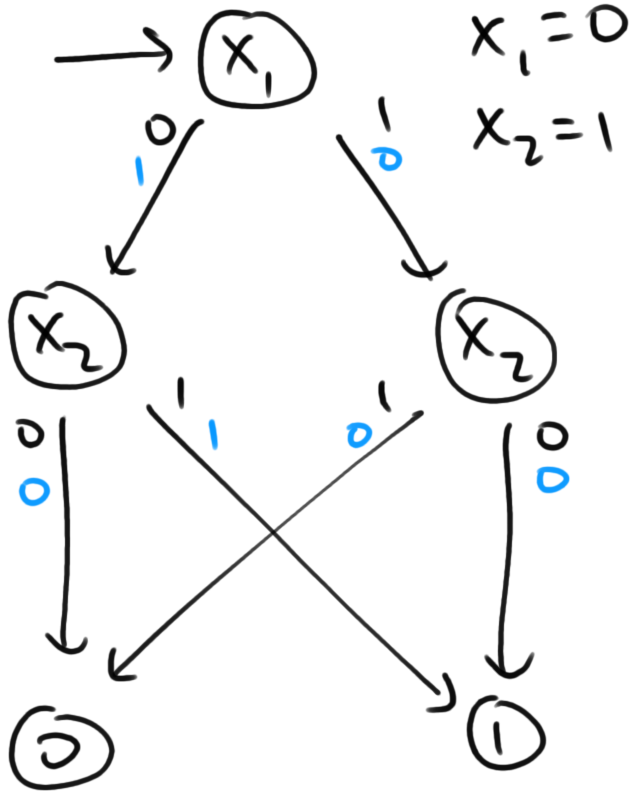
\includegraphics[scale=0.2]{EQ_ROBP_in_BPP1}
  %\qquad
  %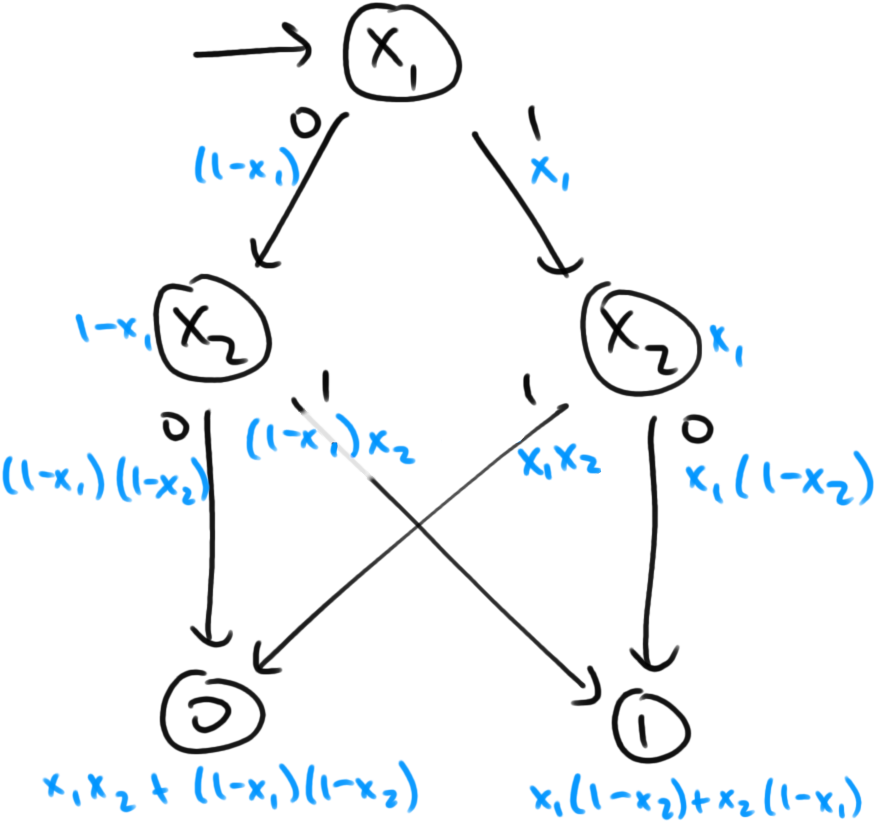
\includegraphics[scale=0.2]{EQ_ROBP_in_BPP2}
\end{example}

More generally, we have the following labeling rules
\begin{center}
  \begin{tikzpicture}[automaton]
    \definecolor{markblue}{rgb}{0.2, 0.5, 1}
    \NewDocumentCommand{\marknode}{m}{\scalebox{0.7}{\color{markblue}#1}}

    \node[state, label=below:{\marknode{\(a + b + c\)}}] (q) {};
    \node[above left=of q] (anode) {};
    \node[above=of q] (bnode) {};
    \node[above right=of q] (cnode) {};

    \path (anode) edge node[swap]{\marknode{\(a\)}} (q);
    \path (bnode) edge node{\marknode{\(b\)}} (q);
    \path (cnode) edge node{\marknode{\(c\)}} (q);
  \end{tikzpicture}
  \qquad
  \begin{tikzpicture}[automaton]
    \definecolor{markblue}{rgb}{0.2, 0.5, 1}
    \NewDocumentCommand{\marknode}{m}{\scalebox{0.7}{\color{markblue}#1}}

    \node[state, label=above:{\marknode{\(a\)}}] (q) {};
    \node[below left=of q] (anode) {};
    \node[below right=of q] (cnode) {};

    \tikzset{inner sep=1pt}
    \path (q) edge node[swap, pos=0.2]{\(\mathtt 0\)} (anode);
    \path (q) edge node[swap, inner sep=1pt, pos=0.5]{\marknode{\(a(1 {-} x_i)\)}} (anode);
    \path (q) edge node[pos=0.2]{\(\mathtt 1\)} (cnode);
    \path (q) edge node[inner sep=1pt, pos=0.5]{\marknode{\(a x_i\)}} (cnode);
  \end{tikzpicture}
  %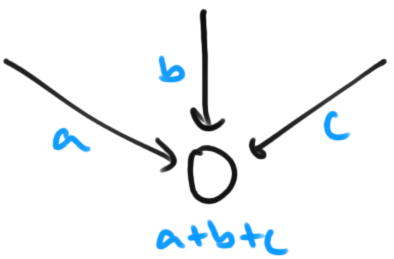
\includegraphics[scale=0.25]{EQ_ROBP_in_BPP3}
  %\qquad
  %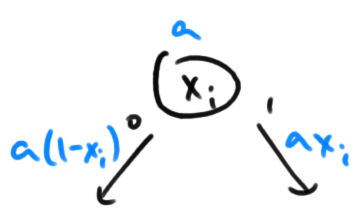
\includegraphics[scale=0.27]{EQ_ROBP_in_BPP4}
\end{center}
Then, the formula the corresponds to the \(\mathtt 1\) output
is the one the represents the \textsf{BP}.

\begin{claim}
  For \textsf{ROBP}s \(B_1\) and \(B_2\) with polynomials \(P_1\) and \(P_2\),
  then over \(r_1, \dots, r_m \in \FF_q\),
  \[
    \PP[P_1(r_1, \dots, r_m) = P_2(r_1, \dots, r_m)] = \begin{cases}
      1 & \text{$B_1$ and $B_2$ are equivalent} \\[-1ex]
      \leq \frac{m}{q} & \text{else}.
    \end{cases}
  \]
\end{claim}
\begin{proof}[Sketch]
  Since \(B_1\) and \(B_2\) are read-once, the degree of
  the polynomials \(P_1\) and \(P_2\) in each variable is at most \(1\).

  Now suppose that \(B_1\) and \(B_2\) are equivalent.
  Note that \(P_1\) and \(P_2\) can be written as sums of
  terms of the form \(y_1 y_2 \dotsm y_m\),
  where \(y_i\) is either \(x_i\) or \(1 - x_i\).
  (If a certain variable \(x_i\) is not on a path,
  we can use the fact that \(1 = x_i + (1 - x_i)\) and expand.)
  Moreover, in this form, the polynomials give us precisely
  the inputs of the \textsf{ROBP}s that output \(1\).
  Therefore, \(P_1\) and \(P_2\) are the same in this case.

  Now suppose that \(B_1\) and \(B_2\) are not equivalent.
  Then note that \(P_1 - P_2 \neq 0\) from looking at
  the representation of \(P_1\) and \(P_2\) with
  terms of the form \(y_1 y_2 \dotsm y_m\) as before.

  The \(\frac{md}{q}\) is from Schwartz-Zippel.
  Since these are read-once \textsf{BP}s, we have \(d = 1\),
  so \(\PP = \frac{m}{q}\).
  We can choose \(q \geq 3m\), so \(\PP \leq \frac{1}{3}\), as desired.
\end{proof}

\begin{corollary}
  \(\textit{EQ}_{\textsf{ROBP}} \in \mathsf{BPP}\).
\end{corollary}


\section{Interactive Proofs}
Consider the problem of graph isomorphism (denoted by \(G_1 \iso G_2\)):
\[
  \textit{ISO} = \set{\angles{G_1, G_2} \mid G_1 \iso G_2}.
\]
It is clear that \(\textit{ISO} \in \mathsf{NP}\) because a certificate
would just be a bijection of the vertices.
However, \textit{ISO} is not known to be
\(\mathsf{NP}\)-hard or in \(\mathsf{P}\).

Suppose that we have two graphs \(G_1\) and \(G_2\).
Also suppose that we have two parties named \(P\) (prover) and \(V\) (verifier).
If \(V\) runs in probabilistic polynomial time,
and \(P\) has unlimited computation power,
then how can \(P\) prove to \(V\) that \(G_1 \iso G_2\) or \(G_1 \ncong G_2\)?

Consider the following protocol:
\begin{enumerate}
  \item \(P\) claims either \(G_1 \iso G_2\) or \(G_1 \not\iso G_2\).
  \item If \(P\) claimed \(G_1 \iso G_2\), then \(P\) provides the certificate,
    and \(V\) checks it.
    \(V\) either \textsc{accepts} or \textsc{rejects} at this case.
  \item If \(P\) claims \(G_1 \not\iso G_2\),
    then \(V\) repeats the following procedure \(N\) times:
  \begin{enumerate}
    \item \(V\) secretly takes one of \(G_1, G_2\) randomly and
      scrambles it to another graph \(G\) isomorphic to the selection.
    \item \(V\) asks \(P\) which of \(G_1\),
      \(G_2\) that \(G\) is isomorphic to.
  \end{enumerate}
  \item If \(P\) gets all of them right,
    then \(V\) \textsc{accepts}, else \textsc{reject}.
\end{enumerate}

Note that if \(P\) lies in the first case,
then \(V\) will know with the certificate.
In the other case, \(V\) will catch the lie with probability \(1 - 2^{-N}\).

\begin{definition}
  Consider two parties \(P\) unlimited computation and
  \(V\) with probabilistic polynomial computation respectively.
  Both exchange messages until \(V\) accepts or rejects. Let
  \[
    \PP[\text{$(V\leftrightarrow P)$ accepts $w$}] \coloneqq
      \PP[\text{$V$ ends up accepting}].
  \]
\end{definition}
\begin{definition}
  Let \(\mathsf{IP}\) (for \vocab{interactive proofs}) be
  \begin{align*}
    \mathsf{IP} \coloneqq \lbrace
      A \mid {}& \text{there exists a protocol $(V \leftrightarrow P)$ where} \\
      {}& w \in A \iff
            \PP[\text{$(V\leftrightarrow P)$ accepts $w$}] \geq \tfrac{2}{3} \\
      {}& \text{$w \notin A \iff
            \PP[\text{$(V\leftrightarrow \tilde P)$ accepts $w$}]
                \leq \tfrac{1}{3}$ for all $\tilde P$}
    \rbrace.
  \end{align*}
\end{definition}

We know that \(\mathsf{NP} \subseteq \mathsf{IP}\) because
the prover can just send the certificate.

We also know that \(\mathsf{BPP} \subseteq \mathsf{IP}\) because
the verifier can tell the prover to go away and just do the problem themself.

It turns out that \(\mathsf{IP} \subseteq \mathsf{PSPACE}\),
but we will not prove this. The idea of the proof is to
explore all possible interactions in polynomial space.
We will prove the weaker statement \(\mathsf{coNP} \subseteq \mathsf{IP}\)
by showing \(\hash\mathit{SAT} \in \mathsf{IP}\).
(Note that \(\hash\mathit{SAT}\) is \(\mathsf{coNP}\)-hard
  because \(\overline{\mathit{SAT}} \polyredu \hash\mathsf{SAT}\)
  by the reduction \(\angles{\phi} \to \angles{\phi, 0}\).)


\end{document}
